\section{Experimental Evaluation}
\label{sec:simulation}

The experiment studies the effect of an increasing penetration rate
of vehicular automation technology.  Suppose human-driven vehicles are
gradually replaced by a particular type of semi-autonomous vehicle or
fully autonomous vehicle until all vehicles become that type.  We examine how
much benefit SemiAIM provides during the transition period.

In this experiment, the traffic consisted of one of the three types of
vehicles we defined in Section~\ref{sec:vehicles} as well as Type A
and Type H vehicles.  We measured the traffic delay as we gradually
increased the ratio of (semi-)autonomous vehicles to human-driven
vehicles (Type H) while keeping the traffic level at 360
vehicles/hour/lane.  As an example, consider the ratio of Type SA-ACC
vehicles.  At the beginning, there are 0\% Type SA-ACC vehicles and
100\% human-driven vehicles, and the ratio is 0.  As the number of
Type SA-ACC vehicles increases, the ratio increases and eventually
becomes 1, which means there are 100\% Type SA-ACC vehicles and 0\%
human-driven vehicles.  We repeated the simulation 30 times for 1800s
during each time.  For each run, we measured the average delay of all
vehicles.  The average delays are shown in Figure~\ref{fig:two360}.
Each data point in the figure is an average of 30 values, and the
error bar is the 95\% confident interval of the average delay.
 
% , and the average delay is the same as Type
% H's.  When the ratio is 1, the traffic has 100\% SA-ACC vehicles and
% 0\% human-driven vehicles, and the average delay is 22.4s.

% When the
% ratio is 0.6, the traffic has 60\% SA-ACC vehicles and 40\%
% human-driven vehicles, and the average delay is 32.9s.  


\begin{figure}
\centering
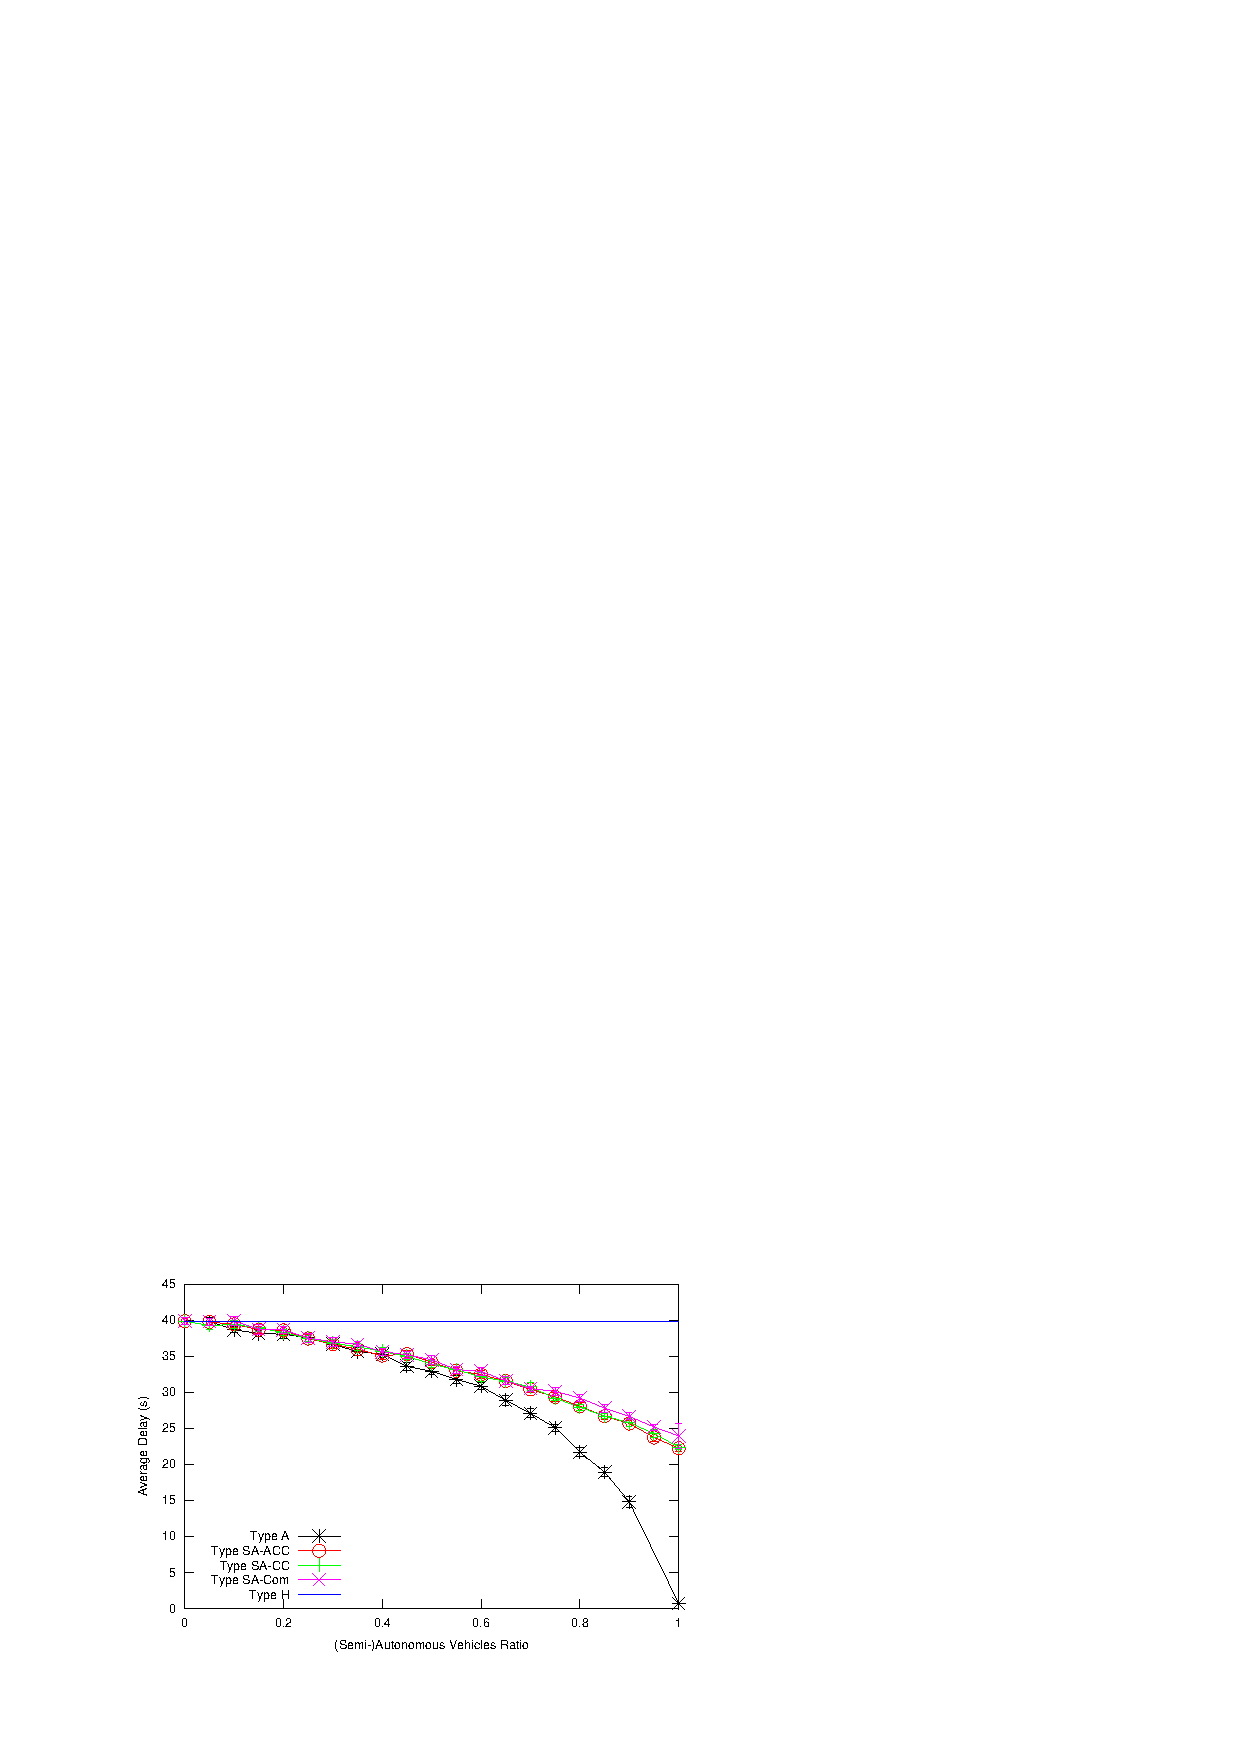
\includegraphics[width=0.9\columnwidth]{figures/figure_1.png}
\caption{(Semi-)Autonomous vehicles vs. Human-Driven vehicles. Traffic
level = 360 vehicles/lane/hour.}
\label{fig:two360}
\vspace{-.2in}
\end{figure}

According to Figure~\ref{fig:two360}, the performance of
semi-autonomous vehicles is very similar to fully autonomous vehicles
when the ratio to human-driven vehicles is below 40\%.  However, when
the ratio increases beyond 40\%, fully autonomous vehicles
increasingly outperform semi-autonomous vehicles.  Previous studies
showed that FCFS-Signal needs at least 90\% of fully autonomous
vehicles in the traffic in order to be fully
effective~\cite{bib:Dresner07Sharing}.  We successfully replicate the
result, observing that the average delay drops rapidly when the
traffic has more than 90\% fully autonomous vehicles, and approaches
zero when all vehicles are fully autonomous.  Semi-autonomous vehicles
cannot achieve the same dramatic decrease in traffic delay, but they,
with the help of SemiAIM, manage to reduce the delay by 46\% (from
39.9s to 22.4s) compared to human-driven vehicles.  As expected, in
the presence of semi-autonomous vehicles, SemiAIM provides significant
advantages even when there are no fully autonomous vehicles on the
road.
Another observation is that both Type SA-ACC and Type SA-CC vehicles
have a significantly lower average delay than Type SA-Com vehicles.
% The difference is consistent with our hypothesis that the use of more
% constrained requests can increase the performance of intersections
% since the footprints of the vehicles are smaller and more vehicles can
% enter the intersection at the same time.  Nonetheless, the difference
% is small because the simulated human drivers in the simulator can
% control their vehicles quite well.
% 
% In reality the difference actually depends on some human drivers needs
% to reserve a large number of tiles, causing a decrease of the traffic
% delay when all vehicles are human-driven.  assumption we made on how
% well human drivers perform. In our simulations,

% This result confirms our hypothesis that while semi-autonomous
% vehicles can significantly bridge the gap between the time when all
% vehicles are human-driven to that when most are autonomous, there will
% likely always remain strong benefits of full autonomy, especially at
% high traffic levels.  



% It is true that semi-autonomy would not ``harm'' normal traffic which
% follows traffic signals, but they have almost no chance to enter the
% intersection in phases other than when the signal is green. This
% condition leads to little or no improvement over traditional traffic
% light policy.



% However, the average delay of
% semi-autonomous vehicles cannot be reduced to nearly zero.  When all
% vehicles are semi-autonomous, the average delay (22.4s) is roughly
% half of the average delay for human-driven vehicles only (39.9s).  

% The last observation is that 
% if there are less than 80\% of vehicles
% that are fully autonomous and more than 20\% of vehicles that are
% human-driven, it is still possible to form a team of semi-autonomous
% vehicles that performs better. Thus, we need at 80\% of fully
% autonomous vehicles in order to guarantee the benefit.

% We expect that
% in the presence of semi-autonomous vehicles, SemiAIM
% will provide significant advantages over FCFS-Signal if we assume that
% semi-autonomous vehicles have to act as fully human-driven vehicles in
% FCFS-Signal.  

% The experiments only compare two types of vehicles at the same
% time---human-driven vehicles (Type H) and the type of vehicles
% specified in the legends.

% As described in the
% legend, the traffic level is 360 vehicles/hour/lane, so it can be
% easily calculated how many vehicles of a certain type are spawned in
% each lane.

% Another observation is that the average delay when all vehicles are
% semi-autonomous (i.e., the ratio is 1) is approximately equal to the
% average delay of fully autonomous vehicles when the ratio is 0.8
% (i.e., 80\% of vehicles are fully autonomous and the remaining 20\%
% are human-driven). Thus 

% Another observation is that if there are less than 80\% of vehicles
% that are fully autonomous and more than 20\% of vehicles that are
% human-driven, it is still possible to form a team of semi-autonomous
% vehicles that performs better. Thus, we need at 80\% of fully
% autonomous vehicles in order to guarantee the benefit.

% To demonstrate the feasibility of SemiAIM as well as evaluate the
% hypothesis that SemiAIM can offer substantial improvements over
% traffic signals and FCFS-Signal,

